%\documentclass[11pt, twoside, titlepage, a4paper, openright]{report}
\documentclass[12pt, oneside, titlepage, a4paper]{report}
\usepackage{graphicx}
\usepackage[english]{babel}
\usepackage[utf8]{inputenc}
\usepackage{algpseudocode}
\usepackage{amsthm}
\usepackage{algorithm}
\usepackage{rotating}
\usepackage{enumerate}
%\usepackage[Lenny]{fncychap}
\usepackage{hyperref}
\hypersetup{
    colorlinks=true,       % false: boxed links; true: colored links
    linkcolor=black,%red,          % color of internal links
    citecolor=black,%green,        % color of links to bibliography
    filecolor=black,%magenta,      % color of file links
    urlcolor=black%cyan           % color of external links
}
\usepackage [a4paper,left=2.5cm,bottom=2.5cm,right=2.5cm,top=3cm]{geometry}
\usepackage{frontespizio}

\newtheorem{mydef}{Definition} % definizioni <-----
%\nofiles 
%\fontoptionnormal 

\usepackage{mathtools}

\frenchspacing

\begin{document}


\begin{frontespizio}
\Universita {Verona}
\Dipartimento {Informatica}
\Corso {Ingegneria e Scienze Informatiche}
\Annoaccademico {2017-2018}
\Titoletto {Tesi di Laurea Magistrale}
\Titolo { \Large {Multi-Robot Task Allocation for logistic applications} }
\Candidato [vr414572]{Davide Zorzi}
\Relatore {Alessandro Farinelli}
\Correlatore{Riccardo Muradore}
\Rientro {1.5cm}
\NCandidato {Candidato}
\end{frontespizio}

%\clearpage\null\thispagestyle{plain}\clearpage
%\newpage

%\preparefrontpage

\tableofcontents

\newpage

\paragraph{Abstract}
\begin*{}
\newline
\newline
Robotics technology has recently matured sufficiently to deploy autonomous
robotic systems for daily use in several applications: from disaster response
to environmental monitoring and logistics.
In this project present and evaluate the principal difference of central and 
distributed allocator task coordinator. 
In these applications we address off-line coordination, by casting the Multi-Robot
logistics problem as a task assignment problem and proposing two solution 
techniques: Cyclic Greedy Strategy Single Robot Single Task (CGS1:1), which is 
a baseline greedy approach, and Cyclic Greedy Strategy Single Robot Multiple Task 
(CGS1:N), which is based on merging task for improve the spend time.
\\
And the last one is address on-line coordiantor, that is based on token passing (TP) approach.
We evaluate the performance of our system in a realistic simulation enviroment
(build with ROS and stage). In particular, in the simulated enviroment we compare
our task assignment approaches with previous off-line and on-line methods.
\newline
\newline
\textbf{Keywords:} Multi-Robot Task Allocator, logistic applications, Multi-Robot
systems, coordination, task assignment

% TODO: primi risultati e considierazioni

\end*{}




\chapter{Introduction}\label{chap:intro}

    \begin{frame}[fragile]{Industrial Logistics}
        The {\bf industrial logistics} is the process of {\bf planning}, {\bf organization}
        and {\bf control} of all the activities of handling and {\bf storage} of goods, which, starting
        from the suppliers and reaching up to the end user, guarantee an adequate
        level of {\bf service} to the customer consistent with the {\bf costs} to it associated

        \begin{figure}[hbt]
            \centering
            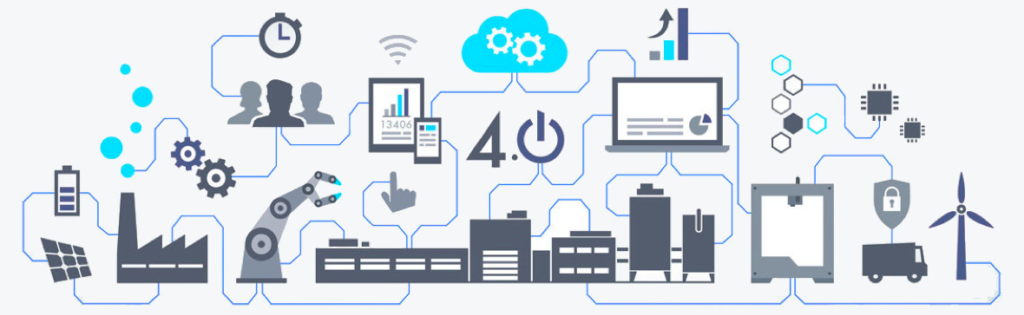
\includegraphics[width=\textwidth]{img/ind4.png}
        \end{figure}
    \end{frame}

    \begin{frame}[fragile]{Multi-Robot Systems for logistic applications}

        \begin{figure}[hbt]
            \centering
            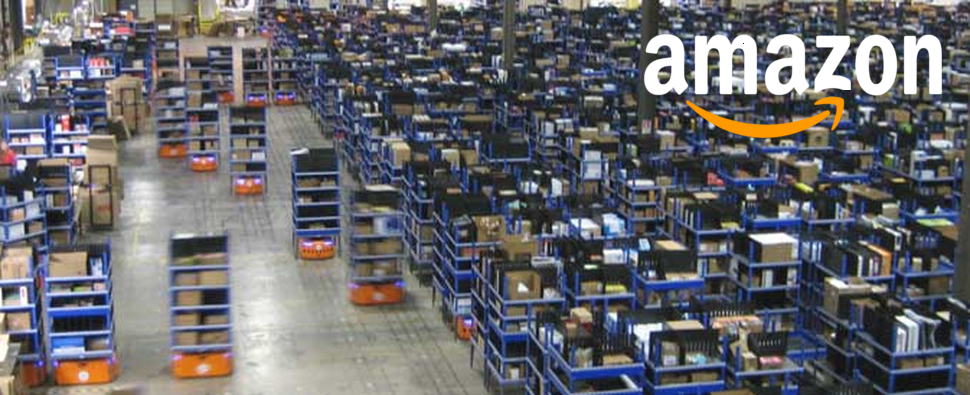
\includegraphics[width=\textwidth]{img/kiva.png}
        \end{figure}
        
        \begin{center}
        Kiva warehouse-management system
        \end{center}
    \end{frame}

    \begin{frame}[fragile]{Thesis contribution}
        \begin{center}
        The contribution of this thesis:
        \end{center}
        \begin{columns}
            \begin{column}{.7\textwidth}
           
            \begin{itemize}
            \item extension of  \texttt{ROS}  package
            \item proposing three tequnique:
            \begin{enumerate}
                \item Single robot : Single task (SR:ST) 
                \item Set Partition Strategy - Single robot : Multiple task (SPS1:N)
                \item Greedy Set Partition Strategy - Single robot : Multiple task (GSP1:N)
            \end{enumerate}
                \item real scenario: Computer Engineering for Industry 4.0 Laboratory (ICE Lab) 
            \end{itemize}
            \end{column}
            \begin{column}{.4\textwidth}
            \begin{figure}
                \subfloat{
\includegraphics[scale=0.45]{img/ros}}\qquad
                \subfloat{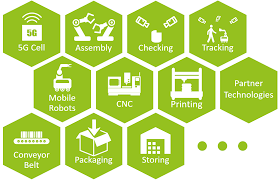
\includegraphics[scale=0.45]{img/ice}}
            \end{figure}
            \end{column}
        \end{columns}
    \end{frame}


    \begin{frame}[fragile]{ICE Laboratory}
        \begin{figure}[hbt]
            \centering
            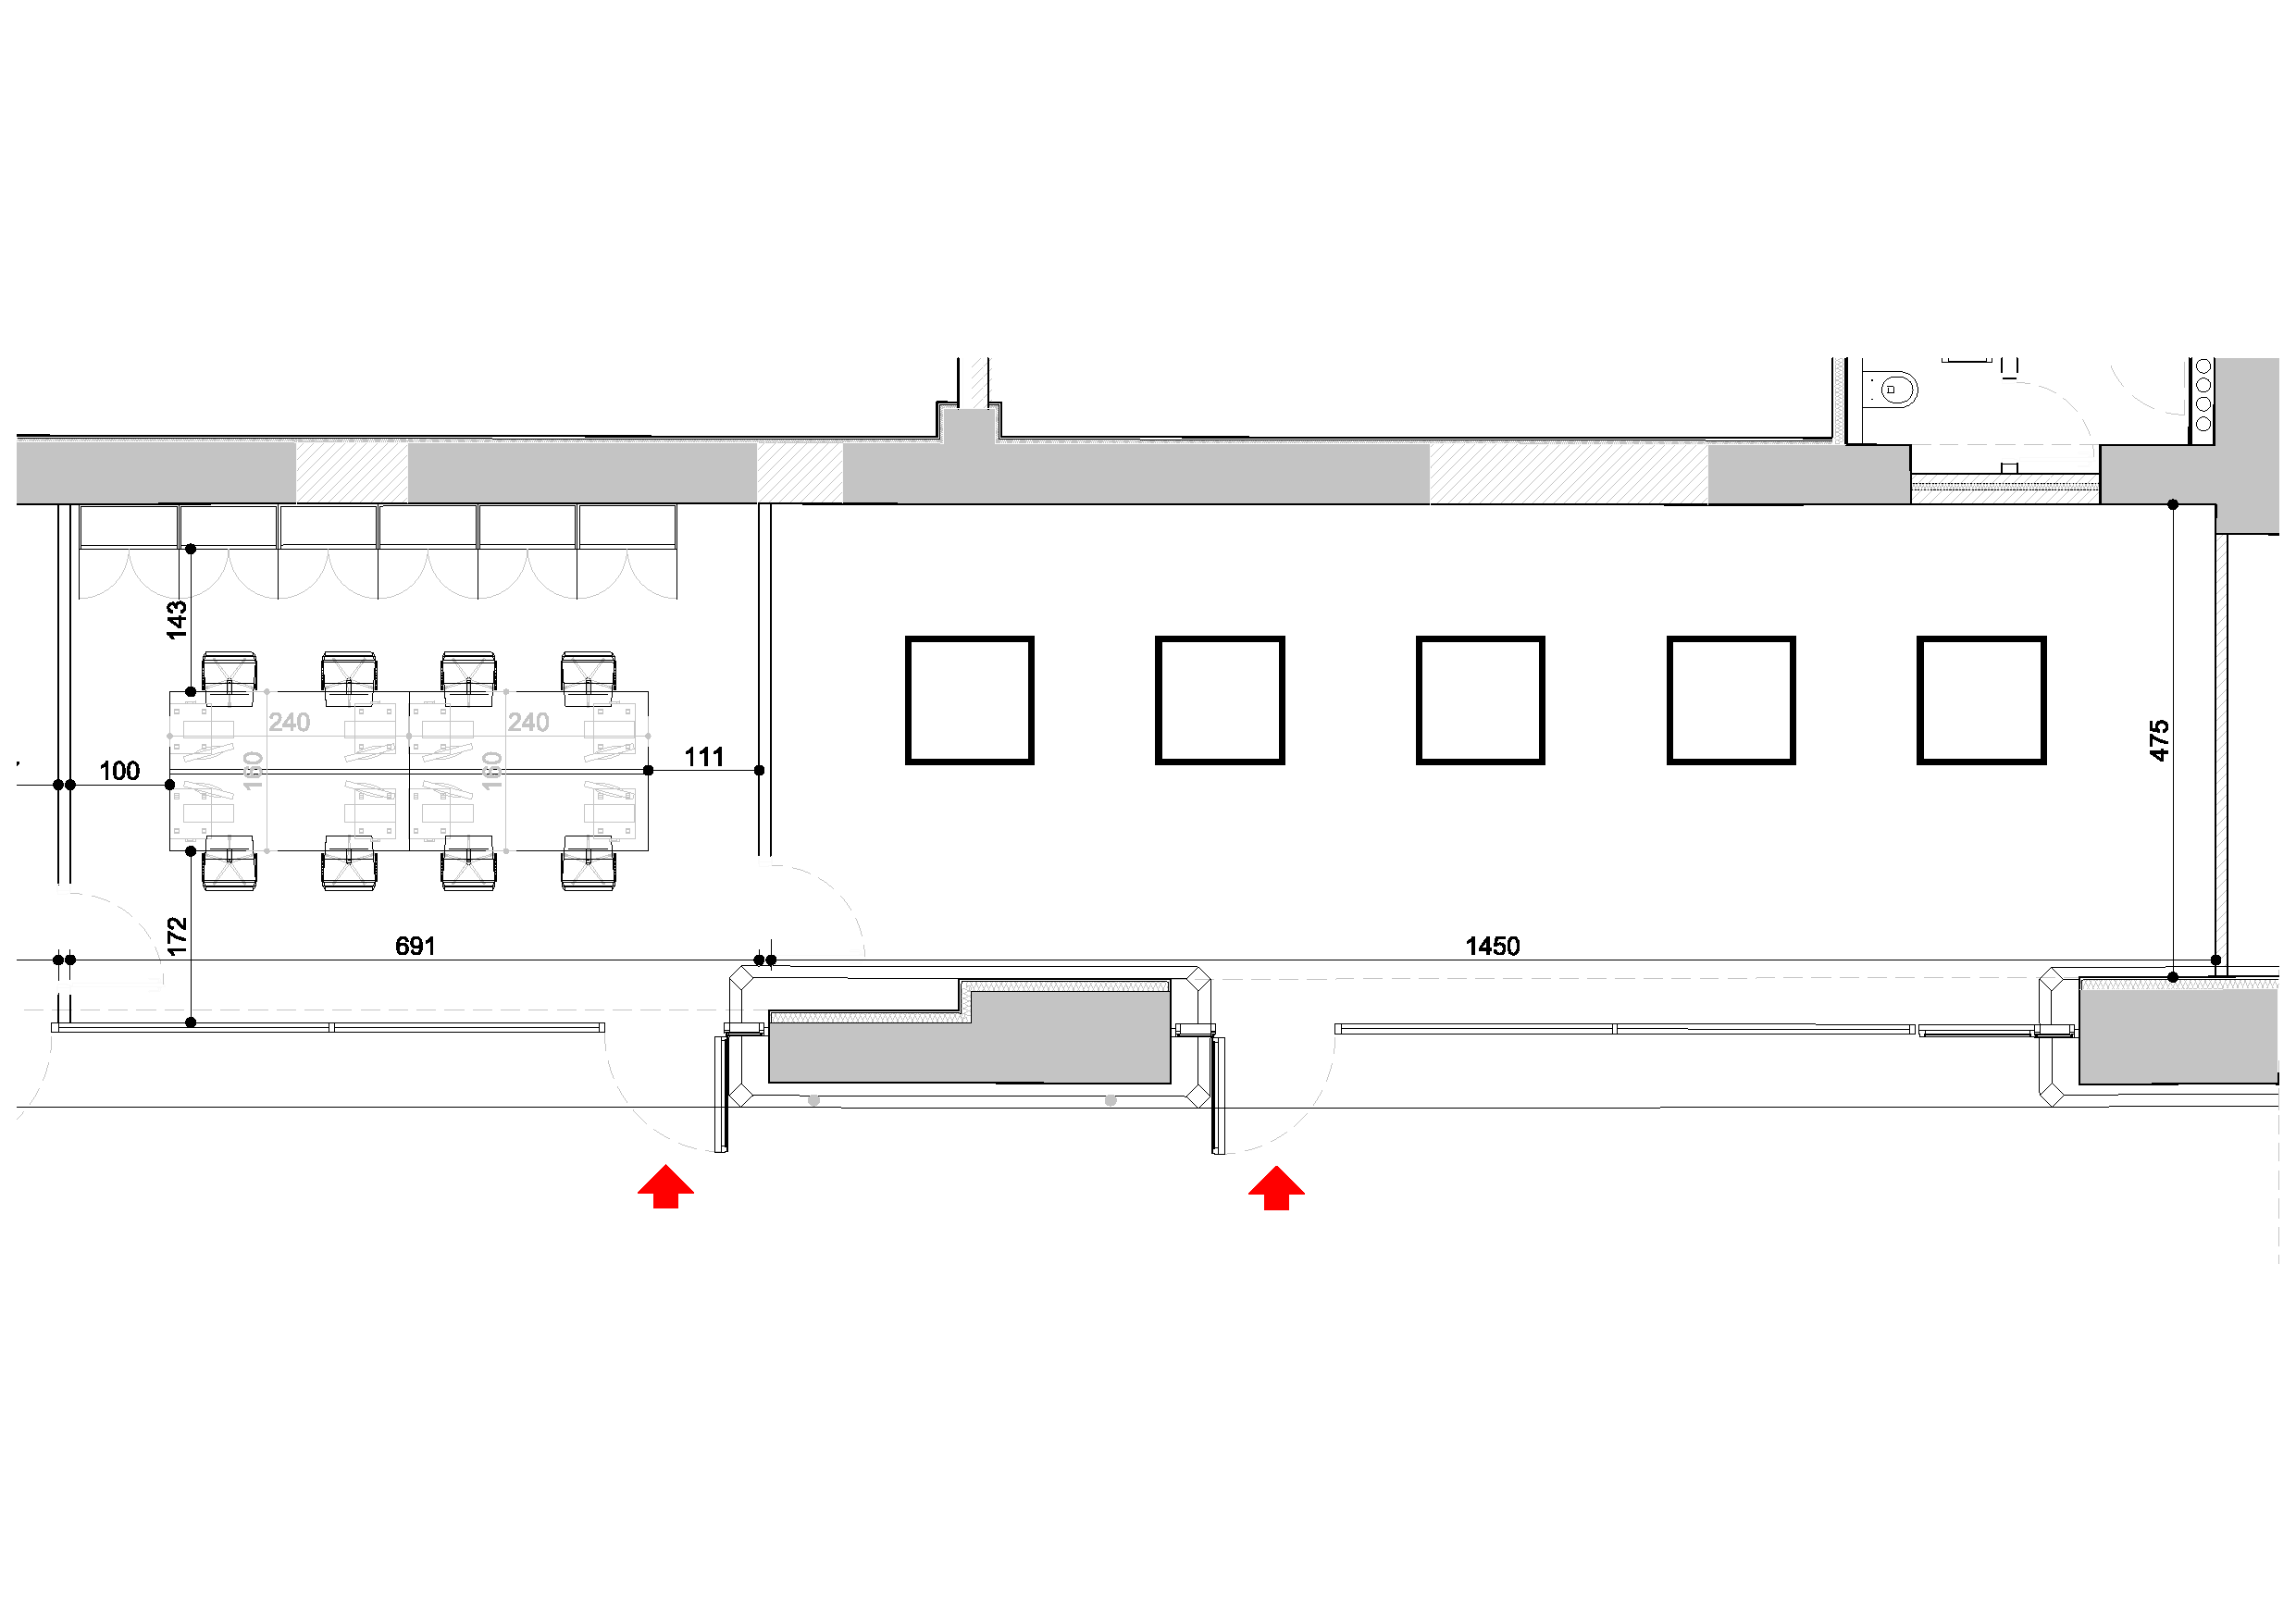
\includegraphics[width=\textwidth]{img/model1}
        \end{figure}
    \end{frame}

    \begin{frame}[fragile]{ICE Laboratory for logistic application}
        \begin{figure}[hbt]
            \centering
            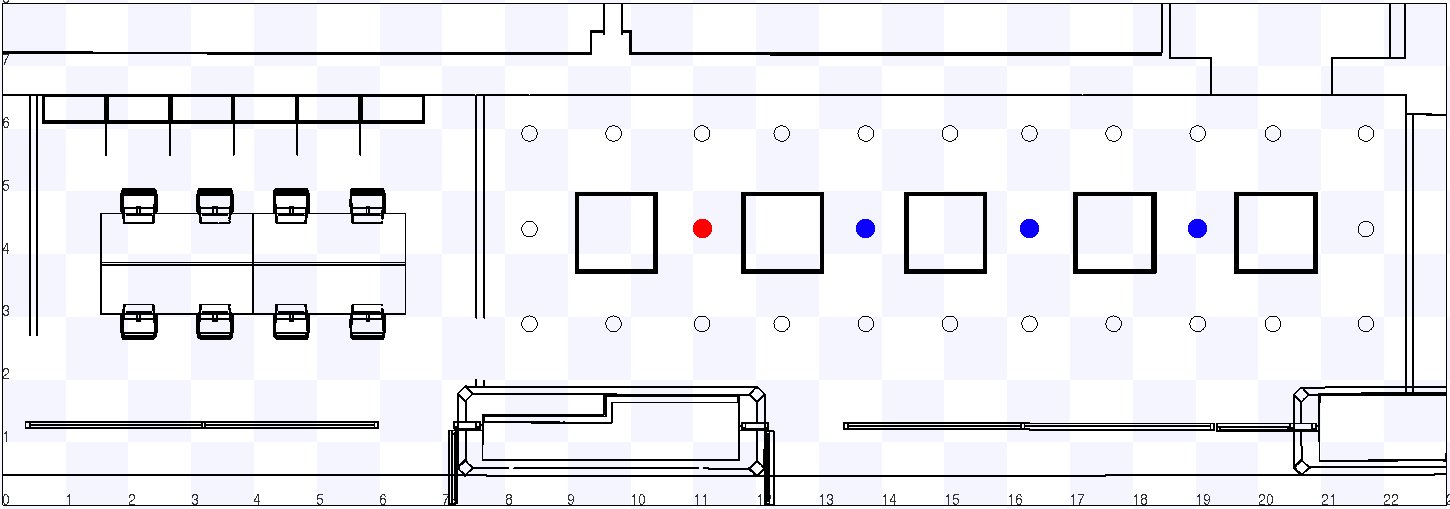
\includegraphics[width=\textwidth]{img/labgrafo}
        \end{figure}

        {\color{red}{$\bullet$}}  Loading bay
        \\
        {\color{blue}{$\bullet$}}  Unloading bays
        \\
        {\color{black}{$\circ$}}  Vertices
    \end{frame}

    \begin{frame}[fragile]{Set Partition Strategy - Single robot : Multiple task (SPS1:N)}
         \begin{columns}
            \begin{column}{.7\textwidth}
                \begin{center}
                    \begin{tabular}{|c|r|c|} \hline
                    \textbf{iteration} & \textbf{partition size} & \textbf{partition} \\ \hline
                    1    & 1    & \{\{a, b, c, d\}\}   \\
                    2    & 2    & \{\{a, b, c\}, \{d\}\}   \\
                    3    & 2    & \{\{a, b, d\}, \{c\}\}   \\
                    4    & 2    & \{\{a, b\}, \{c, d\}\}   \\
                    5    & 3    & \{\{a, b\}, \{c\}, \{d\}\}   \\
                    6    & 2    & \{\{a, c, d\}, \{b\}\}   \\
                    7    & 2    & \{\{a, c\}, \{b, d\}\}   \\
                    8    & 3    & \{\{a, c\}, \{b\},\{d\}\}   \\
                    9    & 2    & \{\{a, d\}, \{b, c\}\}   \\
                    10   & 2    & \{\{a\}, \{b, c, d\}\}   \\
                    11   & 3    & \{\{a\}, \{b, c\}, \{d\}\}   \\
                    12   & 3    & \{\{a, d\}, \{b\}, \{c\}\}   \\
                    13   & 3    & \{\{a\}, \{b, d\}, \{c\}\}   \\
                    14   & 3    & \{\{a\}, \{b\}, \{c, d\}\}   \\
                    15   & 4    & \{\{a\}, \{b\}, \{c\},\{d\}\}   \\ \hline       
                    \end{tabular}
                  \end{center}
            \end{column}
            \begin{column}{.4\textwidth}
            \begin{figure}
                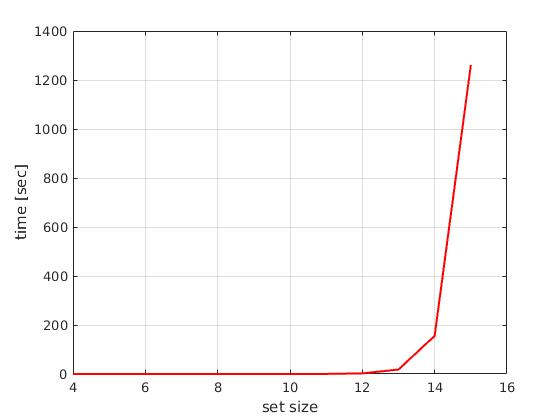
\includegraphics[width=\textwidth]{img/exp}
            \end{figure}
            \end{column}
        \end{columns}
    \end{frame}

    \begin{frame}[fragile]{Greedy Set Partition Strategy - Single robot : Multiple task (GSP1:N)}
    \end{frame}

    \begin{frame}[fragile]{ROS package Logistic\_sim}
        \begin{figure}[hbt]
            \centering
            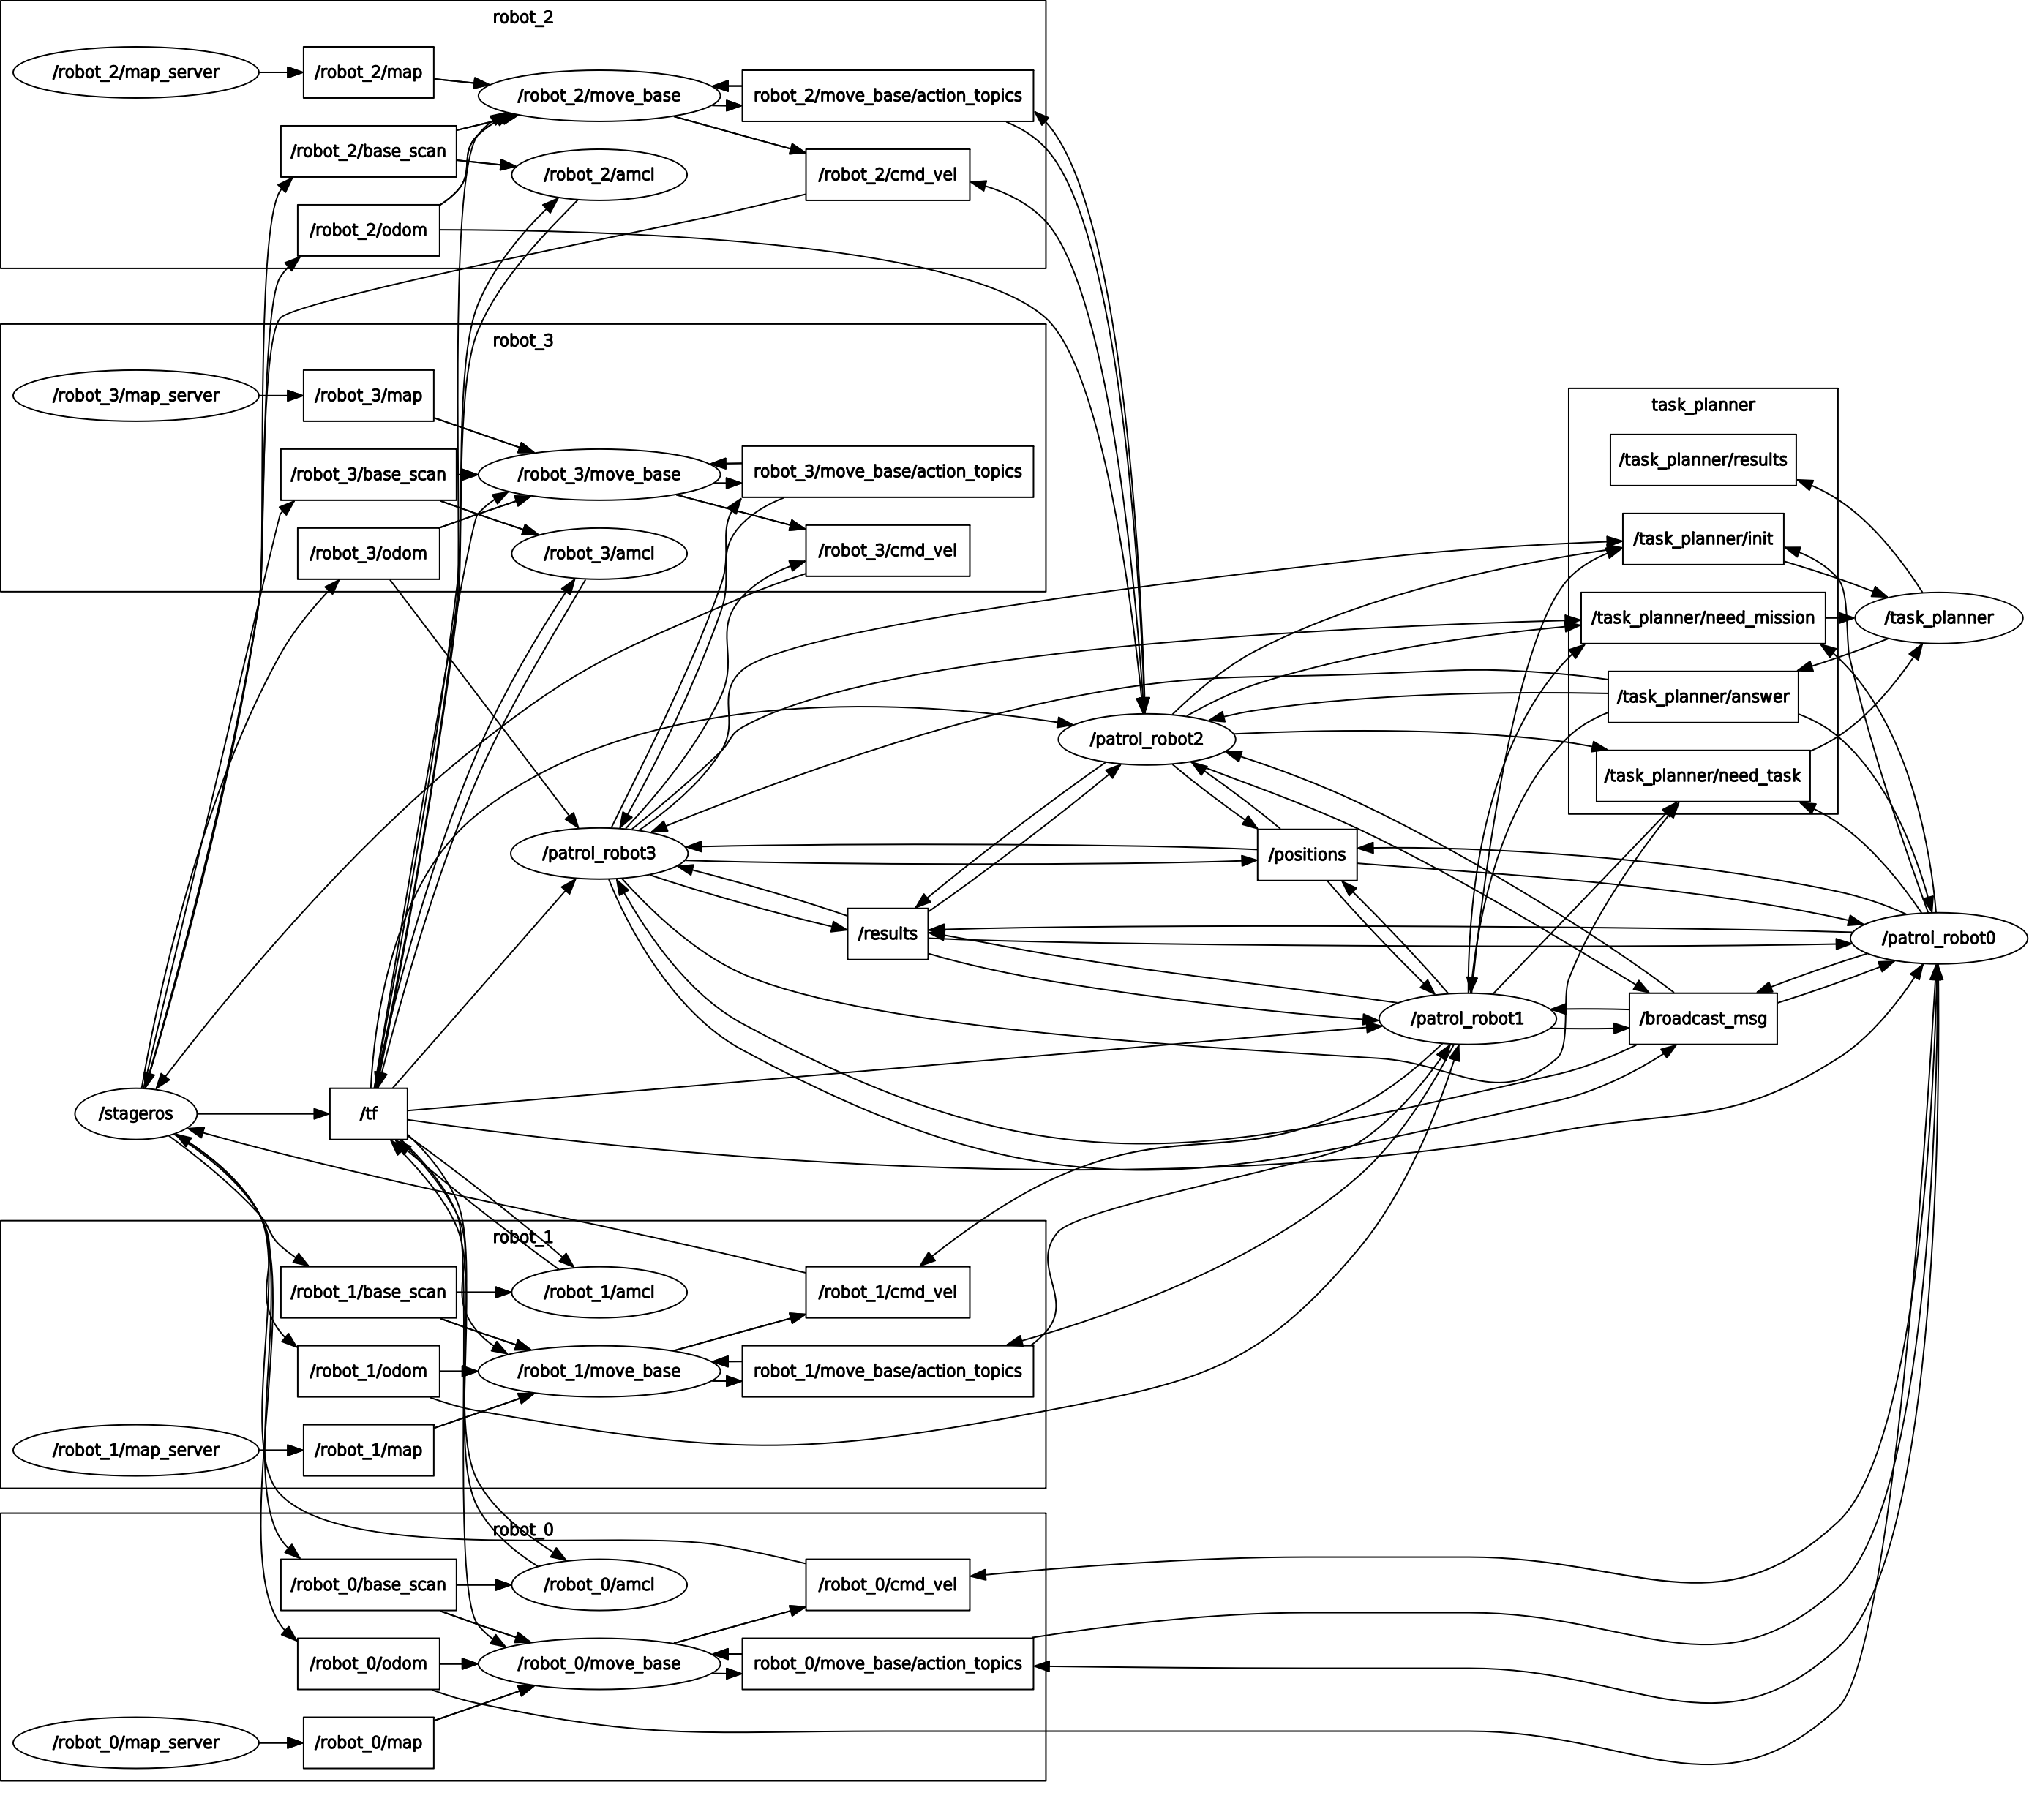
\includegraphics[scale=0.12]{img/rosgraph}
        \end{figure}
    \end{frame}

    \begin{frame}[fragile]{Empirical Results}
    \end{frame}

    \begin{frame}[fragile]{Video}
    \end{frame}

    \begin{frame}[fragile]{Conclusions and Future Work}
    \end{frame}









\chapter{Background and Related Works}\label{chap:related}

\chapter{Problem}\label{chap:problem}

\chapter{Solution}\label{chap:solution}

\chapter{Experiments}\label{chap:experiments}

\chapter{Conclusions}\label{chap:conclusions}

\chapter*{Acknowledgements}
\addcontentsline{toc}{chapter}{\protect\numberline{}Acknowledgements}

%\bibliographystyle{splncs03}
%\bibliography{biblio}

\end{document}
